\section{Formal Analysis using Alloy}
Alloy is a declarative language commonly used to describe, model, and verify complex systems.
Its objective is creating small models and checking their correctness, using the power of first order logic.
We used Alloy to model and verify the behavior of specific parts of the application.

\subsection{Queue Modeling}
Queue management is one of the most critical aspects of the application.
We implemented the concept of queue as a set of ordered Tickets.
We made the assumption that each customer will stay at least one unit of time inside of the store to be able to model it through Alloy Int variables. 
To create a fully populated world we used one fact to have all the slot assigned to at least one ticket. 
We checked that no slot inside of the store is assigned to multiple people at the same time, by respecting the registered entrance and exit time. 

\lstinputlisting[language=C]{alloy/queue.als}
\begin{figure}[H]
    \centering
    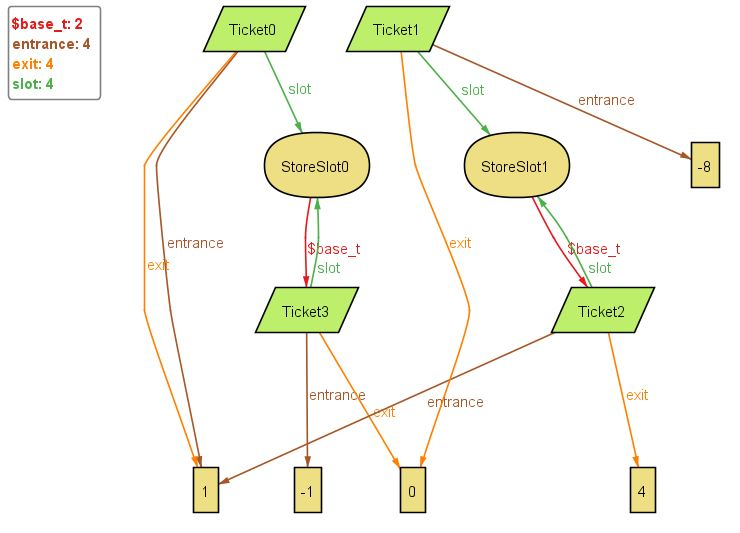
\includegraphics[width=1\textwidth]{alloy/Line_Alloy.JPG}
    %\caption{Enter Store from Queue Sequence Diagram}
\end{figure}

\subsection{Reservation Modeling}
Reservations are another critical aspect of the applications.
Users who make a reservation expect to shop at the specific time of the reservation.
In extreme cases reservations can be automatically cancelled by the system.
This should happen only in case of another user taking too long to shop.
The objective of this Alloy model is to verify that the presence of two concurent reservations at the same slot implies that one of the two has been cancelled by the system.
\lstinputlisting[language=C]{alloy/reservations.als}
\begin{figure}[H]
    \centering
    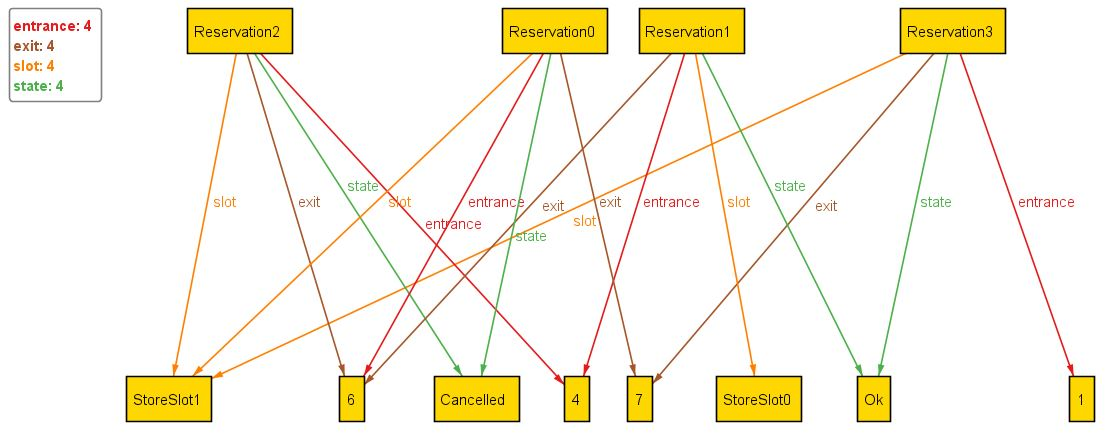
\includegraphics[width=1\textwidth]{alloy/Reservation_Alloy.JPG}
    %\caption{Enter Store from Queue Sequence Diagram}
\end{figure}
